% 研究方法：實驗一包含 Baseline 與集成；實驗二為 FS 集成。
\chapter{研究方法}\label{chap:method}
\begingroup
\setlength{\emergencystretch}{2em}
\clubpenalty=10000
\widowpenalty=10000
\displaywidowpenalty=10000

\section{研究架構}\label{sec:method-framework}

本研究以具有時間資訊的不平衡分類資料為對象，透過歷史模型保留與近期模型加入，探討兩階段集成式持續學習，並評估集成規則與特徵選取的影響。本節先說明通用架構，實際資料與年份配置列於第~\ref{sec:method-data}~節。

每筆輸入包含特徵、分類標籤與觀測時間，可表示為 \(\{(x_i,y_i,t_i)\}_{i=1}^{n}\)。其中，\(n\) 是樣本數，\(x_i\) 是特徵向量，\(y_i\in\{0,1\}\) 是分類標籤，\(t_i\) 是觀測時間。同一個體若有多筆紀錄，另保留識別碼供配對。Old／New 的期間長度、驗證方式與分類器可依應用設定。以 \(\mathcal{O}\) 表示歷史模型池、\(\mathcal{N}\) 表示近期新增模型，框架的更新由 \(\mathcal{O}\) 擴充至 \(\mathcal{O}\cup\mathcal{N}\)，再以驗證資料決定成員與門檻；Old3 與 New3 分別作為只保留單一期間的控制組。實作在同一離線實驗中重建各設定，以模擬這次模型池更新，沒有將多次線上部署或連續更新當成已觀察結果。

實驗安排如圖~\ref{fig:method-overview} 與表~\ref{tab:method-stages}。實驗一包含單一分類器 Baseline 與 Old／New 集成比較；實驗二沿用集成條件，加入特徵選取，並以完整特徵結果為對照。流程中的正類代表應用所關注的類別，各模型依所屬資料分區重新訓練。

\begingroup
\small
\setstretch{1.15}
\setlength{\tabcolsep}{4pt}
\renewcommand{\arraystretch}{1.25}
\setlength{\LTleft}{0pt plus 1fill}
\setlength{\LTright}{0pt plus 1fill}
\begin{longtable}{@{}>{\raggedright\arraybackslash}p{\dimexpr 0.18\linewidth-1.0800\tabcolsep\relax}>{\raggedright\arraybackslash}p{\dimexpr 0.28\linewidth-1.6800\tabcolsep\relax}>{\raggedright\arraybackslash}p{\dimexpr 0.28\linewidth-1.6800\tabcolsep\relax}>{\raggedright\arraybackslash}p{\dimexpr 0.26\linewidth-1.5600\tabcolsep\relax}@{}}
\caption{兩項實驗之研究架構與比較目的}\label{tab:method-stages}\\
\toprule
\textbf{實驗} & \textbf{主要變動因素} & \textbf{比較目的} & \textbf{實驗間之銜接} \\
\midrule
\endfirsthead
\multicolumn{4}{c}{表~\thetable（續）}\\
\toprule
\textbf{實驗} & \textbf{主要變動因素} & \textbf{比較目的} & \textbf{實驗間之銜接} \\
\midrule
\endhead
\midrule
\multicolumn{4}{r}{續下頁}\\
\endfoot
\bottomrule
\endlastfoot
實驗一：Baseline 與集成比較 & 分類器、訓練期間、採樣方式及模型組成 & 建立單模型基準，分析 Old／New 模型的集成方式 & 提供實驗二未進行 FS 的集成對照 \\
\addlinespace[2pt]
實驗二：FS 集成比較 & 特徵選取方法及保留數 & 比較加入 FS 後的集成分類效能 & 沿用實驗一集成設定，進行同條件配對比較 \\*
\end{longtable}
\noindent{\footnotesize (資料來源：本研究整理)}
\endgroup
\begin{figure}[htbp]
\centering
\begingroup
\small
\setstretch{1.12}
\setlength{\fboxsep}{8pt}
\begin{tabular}{@{}c@{}}
\fbox{\parbox{0.88\linewidth}{\centering 具有時間資訊的分類資料\\
定義觀測單位與正類；依時間劃分擬合、驗證與測試用途}}\\[3pt]
\(\Downarrow\)\\[3pt]
\fbox{\parbox{0.88\linewidth}{\centering\textbf{實驗一：Baseline 與集成分類器比較}\\[4pt]
Baseline：分類器、Old／New／Retrain、採樣策略之比較\\
\(\Downarrow\)\\
以固定 XGBoost 建立 Old 三模型與 New 三模型\\
比較靜態集成、DCS 與 DES}}\\[3pt]
\(\Downarrow\)\\[3pt]
\fbox{\parbox{0.88\linewidth}{\centering\textbf{實驗二：特徵選取集成分類器比較}\\[4pt]
沿用集成比較之資料分區、分類器種類與採樣方式\\
以 Old 擬合資料選取特徵，再採樣並重新建立六模型池\\
比較加入 FS 前後的固定方法與驗證選模程序}}\\[3pt]
\(\Downarrow\)\\[3pt]
\fbox{\parbox{0.88\linewidth}{\centering 驗證決策固定後，評估保留的較晚期間測試資料\\
主要報告 AUC、F1-score 與 Recall}}
\end{tabular}
\endgroup
\caption{本研究兩項實驗之整體架構}\label{fig:method-overview}
\par\smallskip{\footnotesize (資料來源：本研究)\par}
\end{figure}

模型建立後，先完成驗證決策，再評估保留的測試資料。指標與比較規則統一於第~\ref{sec:method-validation}~節說明。

\clearpage
\section{實驗資料與配置}\label{sec:method-data}

本研究使用第一章介紹的美國企業年度財務資料進行實證。以下說明資料版本、分類標籤、欄位與時間切分，作為後續兩項實驗的共同依據。

\subsection{資料來源與標籤定義}\label{sec:method-label}

資料研究背景參照 Lombardo 等人\autocite{lombardo2022bankruptcy}，實際採作者於 2024 年 4 月 10 日更新的公開版本\autocite{sowide-bankruptcy-data}。資料涵蓋 1999--2018 年，共有 78,682 筆紀錄、8,971 個匿名公司識別碼及 18 個財務特徵。公開說明記載 8,262 家公司，與檔內識別碼數不同，本文依實際資料計數；版本核對詳見附錄~\ref{sec:appendix-data-fs}。

原始欄位 \nolinkurl{status_label} 記錄公司的最終狀態：609 個識別碼為 \nolinkurl{failed}，其所有年度共 5,220 筆紀錄都標為破產，占 6.63\%。這種最終狀態標籤無法看出公司在哪一年破產，較早年度的紀錄也帶有日後才知道的結果。

因此，本研究的主要標籤改為回溯重建的事件代理標籤：破產公司只有最後一個觀測年度記為正類 1，作為推定下一年度事件的代理；該公司較早年度與所有存續公司的紀錄均為 0。全資料共有 609 筆代理事件，占 0.77\%。本研究將年度 \(t\) 的標籤可用時間設為 \(t+1\)，各分區依此規則檢查其在測試期開始時是否成熟。這是重建協定的年度可用性假設；公開檔沒有可逐筆核對的破產申請日期與財報公開時間，因此不能當成已驗證的實際資訊到達日。

最終狀態標籤保留為對照。兩種標籤使用相同資料列、分區、模型池與選擇規則，只改變目標欄位；對照結果於第~\ref{sec:results-label}~節呈現。

\subsection{欄位與資料品質}

本研究以公司年度紀錄為觀測單位。公司識別碼、年度及標籤只供分區、配對與檢核，不作預測輸入。同一公司可能跨擬合與測試年份出現，因此本研究評估較晚年度的狀態分類，不將結果解釋為對未見公司的驗證。

載入資料時檢查公司與年度組合是否重複，並確認 18 個財務欄位的有效值。目前資料未出現重複公司年度紀錄、遺失值或無限值，因此沒有因這些問題刪除紀錄。流程仍保留平均數補值器，以維持各設定相同的前處理順序。補值與標準化的參數均依各實驗允許的擬合分區估計。

模型只使用 X1--X18，欄位意義見表~\ref{tab:method-feature-dictionary}。2024 年公開版的欄位順序及數值與 2022 年版不同，本文依公開研究附件的欄位名稱及跨版本數值對照整理，未直接沿用 2022 年文獻表中的 X 編號\autocite{sowide-financial-supplement}。本研究保留實際使用版本的數值及欄位順序，未另依舊版倍率換算。公司識別碼、年度、標籤及產業分類均不作預測特徵，也未新增財務比率、股價或落後期特徵。

\clearpage
\begingroup
\small\setstretch{1.12}\setlength{\tabcolsep}{4pt}
\begin{longtable}{@{}>{\raggedright\arraybackslash}p{0.15\linewidth}>{\raggedright\arraybackslash}p{0.77\linewidth}@{}}
\caption{本研究使用之財務特徵}\label{tab:method-feature-dictionary}\\
\toprule
欄位 & 財務項目 \\
\midrule\endfirsthead
\multicolumn{2}{c}{表~\thetable（續）}\\\toprule
欄位 & 財務項目 \\
\midrule\endhead
\midrule\multicolumn{2}{r}{續下頁}\\\endfoot
\bottomrule\endlastfoot
X1 & 流動資產 \\
X2 & 資產總額 \\
X3 & 銷貨成本 \\
X4 & 長期負債總額 \\
X5 & 折舊與攤銷 \\
X6 & 稅息前盈餘（EBIT） \\
X7 & 稅息折舊攤銷前盈餘（EBITDA） \\
X8 & 毛利 \\
X9 & 存貨 \\
X10 & 流動負債總額 \\
X11 & 淨利 \\
X12 & 保留盈餘 \\
X13 & 應收款項總額 \\
X14 & 營收總額 \\
X15 & 市值 \\
X16 & 負債總額 \\
X17 & 銷貨淨額 \\
X18 & 營業費用總額 \\
\end{longtable}
\noindent{\footnotesize (資料來源：本研究依作者公開研究附件之欄位名稱與跨版本資料對照整理\autocite{sowide-financial-supplement})\par 本表使用本研究實際版本的順序；X14 與 X17 在目前公開檔中的數值相同，名稱依發布附件保留。}
\endgroup

\subsection{資料用途與驗證分區}

各年度的紀錄數與標籤比例列於附錄~\ref{sec:appendix-data-fs}，兩項實驗的分區與驗證用途整理於表~\ref{tab:method-split-summary}。

\begingroup
\small
\setstretch{1.15}
\setlength{\tabcolsep}{4pt}
\renewcommand{\arraystretch}{1.25}
\setlength{\LTleft}{0pt plus 1fill}
\setlength{\LTright}{0pt plus 1fill}
\begin{longtable}{@{}>{\raggedright\arraybackslash}p{\dimexpr 0.13\linewidth-0.7800\tabcolsep\relax}>{\raggedright\arraybackslash}p{\dimexpr 0.34\linewidth-2.0400\tabcolsep\relax}>{\raggedright\arraybackslash}p{\dimexpr 0.31\linewidth-1.8600\tabcolsep\relax}>{\raggedright\arraybackslash}p{\dimexpr 0.22\linewidth-1.3200\tabcolsep\relax}@{}}
\caption{兩項實驗資料與驗證設定摘要}\label{tab:method-split-summary}\\
\toprule
\textbf{比較部分} & \textbf{實際擬合資料} & \textbf{驗證用途} & \textbf{測試資料} \\
\midrule
\endfirsthead
\multicolumn{4}{c}{表~\thetable（續）}\\
\toprule
\textbf{比較部分} & \textbf{實際擬合資料} & \textbf{驗證用途} & \textbf{測試資料} \\
\midrule
\endhead
\midrule
\multicolumn{4}{r}{續下頁}\\
\endfoot
\bottomrule
\endlastfoot
實驗一：Baseline & Old：1999–2011；New：2012–2013；Retrain：兩者合併 & 2014 年全部資料，供超參數與門檻決定 & 2015–2018 年 \\
\addlinespace[2pt]
實驗一：集成 & Old-fit：1999–2011；New-fit：2012–2013 & 2014 年等分為 DSEL 與 Calibration & 2015–2018 年 \\
\addlinespace[2pt]
實驗二：FS 集成 & 同實驗一之集成比較；前處理及特徵選取僅擬合 Old-fit & 同實驗一之集成比較，固定資料列分配 & 2015–2018 年 \\*
\end{longtable}
\noindent{\footnotesize (資料來源：本研究整理)}
\endgroup


\clearpage
\subsection{時間視窗與資料配置}\label{sec:method-time-window}

滑動視窗可用來描述框架在時間向前推進時的資料配置：對每一個預測時點，以較早期間建立 Old／New 模型，以獨立的驗證資料決定模型組合與門檻，再評估更晚的 Test；時點前移後，相同規則套用於下一個視窗。各視窗均須重新遵守資料可用時間與擬合邊界，不能把未來標籤提前用於模型建立。

圖~\ref{fig:method-time-window} 上半部示範視窗等距前移，下半部列本研究實際採用的固定配置。這張圖用於說明時間安排，不代表兩項實驗已執行逐年更新模型的滑動視窗評估。本研究的集成與 FS 模型固定使用 Old-fit 1999--2011 年、New-fit 2012--2013 年及 2014 年驗證，測試 2015--2018 年；測試年度之間沒有重新訓練。Baseline 使用相同的年份配置，只把 2014 年整年作為驗證資料。

\begin{figure}[H]
\centering
\includegraphics[width=\linewidth]{figures/time-window-concept.png}
\caption{通用滑動視窗概念與本研究固定年份配置}\label{fig:method-time-window}
\par\smallskip{\footnotesize (資料來源：本研究)\par 上半部為時間配置示意，Val. 表示驗證資料；區段寬度不表示本研究的年份數。下半部之 DSEL 與 Calibration 均來自 2014 年，兩者沒有年內先後順序。\par}
\end{figure}

\clearpage

\section{實驗一：Baseline 與集成分類器比較}\label{sec:method-experiment1}

實驗一先觀察單一分類器使用哪些年度資料、搭配何種採樣方式時有較好的表現，再比較六模型池的整合方式。事件標籤的 Baseline 與集成部分使用相同的資料列、標籤、擬合年份與 Test；差別在於 Baseline 以 2014 年整年調參，集成則把 2014 年分成 DSEL 與 Calibration，且池內模型使用預設參數。

\subsection{Baseline 分類器比較}\label{sec:method-phase1}

Baseline 的流程如圖~\ref{fig:method-baseline}。候選分類器涵蓋 XGBoost、LightGBM、Random Forest、Logistic Regression、TabM 與 TabICL 六種；各自使用 Old、New 或合併資料，搭配四種採樣。四種傳統分類器已完成事件標籤實驗，兩種深度學習分類器先保留既有結果，事件標籤數據待更新，兩批數值分表呈現。
\subsubsection{分類器與超參數設定}\label{sec:method-phase1-params}

事件標籤結果比較 XGBoost、LightGBM、Random Forest 與 Logistic Regression 四種傳統分類器。每個「分類器 \ensuremath{\times} 訓練策略 \ensuremath{\times} 採樣」組合各評估 24 組候選參數：候選 0 為集成池使用的預設參數，其餘 23 組依固定亂數從表~\ref{tab:method-ml-search} 的候選集合抽出，不窮舉全部排列。各候選以種子 42 擬合，依 2014 年驗證資料的 ROC-AUC 選參；選定後以十個種子重新訓練，並以同一驗證資料的 F1-score 決定門檻。測試資料不參與上述決策。TabM 與 TabICL 的方法及既有設定另見下節；其事件標籤版本尚未完成，暫列結果不套用本段的 24 候選與十種子完成狀態。

\clearpage
\begingroup
\footnotesize
\setstretch{1.1}
\setlength{\tabcolsep}{4pt}
\renewcommand{\arraystretch}{1.15}
\setlength{\LTleft}{0pt plus 1fill}
\setlength{\LTright}{0pt plus 1fill}
\begin{longtable}{@{}>{\raggedright\arraybackslash}p{\dimexpr 0.2100\linewidth-0.8400\tabcolsep\relax}>{\raggedright\arraybackslash}p{\dimexpr 0.3100\linewidth-1.2400\tabcolsep\relax}>{\raggedright\arraybackslash}p{\dimexpr 0.4800\linewidth-1.9200\tabcolsep\relax}@{}}
\caption{Baseline 傳統分類器之超參數候選集合}\label{tab:method-ml-search}\\
\toprule
\textbf{分類器} & \textbf{參數項目} & \textbf{超參數候選值} \\
\midrule
\endfirsthead
\multicolumn{3}{c}{表~\thetable（續）}\\
\toprule
\textbf{分類器} & \textbf{參數項目} & \textbf{超參數候選值} \\
\midrule
\endhead
\midrule
\multicolumn{3}{r}{續下頁}\\
\endfoot
\bottomrule
\endlastfoot
\multirow[t]{9}{=}{XGBoost} & n\_\allowbreak{}estimators & 100、300、500、800、1000 \\*
\addlinespace[1pt]
 & learning\_\allowbreak{}rate & 0.01、0.03、0.05、0.1、0.2 \\*
\addlinespace[1pt]
 & max\_\allowbreak{}depth & 3、5、7、10 \\*
\addlinespace[1pt]
 & min\_\allowbreak{}child\_\allowbreak{}weight & 1、3、5、20、50 \\*
\addlinespace[1pt]
 & subsample & 0.7、0.85、1.0 \\*
\addlinespace[1pt]
 & colsample\_\allowbreak{}bytree & 0.7、0.85、1.0 \\*
\addlinespace[1pt]
 & gamma & 0.0、0.1、0.2 \\*
\addlinespace[1pt]
 & reg\_\allowbreak{}alpha & 0.0、0.1、1.0 \\*
\addlinespace[1pt]
 & reg\_\allowbreak{}lambda & 0.5、1.0、3.0、10.0 \\
\addlinespace[1pt]
\multirow[t]{9}{=}{LightGBM} & num\_\allowbreak{}leaves & 31、50、100、150 \\*
\addlinespace[1pt]
 & max\_\allowbreak{}depth & 5、7、10、15、-1 \\*
\addlinespace[1pt]
 & learning\_\allowbreak{}rate & 0.01、0.03、0.05、0.1、0.2 \\*
\addlinespace[1pt]
 & n\_\allowbreak{}estimators & 100、200、500、800、1000 \\*
\addlinespace[1pt]
 & min\_\allowbreak{}child\_\allowbreak{}samples & 20、50、100 \\*
\addlinespace[1pt]
 & subsample & 0.7、0.85、1.0 \\*
\addlinespace[1pt]
 & colsample\_\allowbreak{}bytree & 0.7、0.85、1.0 \\*
\addlinespace[1pt]
 & reg\_\allowbreak{}alpha & 0.0、0.1、1.0 \\*
\addlinespace[1pt]
 & reg\_\allowbreak{}lambda & 0.0、0.1、1.0、3.0 \\
\addlinespace[1pt]
\multirow[t]{5}{=}{Random Forest} & n\_\allowbreak{}estimators & 200、400、600、800 \\*
\addlinespace[1pt]
 & max\_\allowbreak{}depth & None、8、12、16、20、24、32 \\*
\addlinespace[1pt]
 & min\_\allowbreak{}samples\_\allowbreak{}leaf & 1、2、4、8、16 \\*
\addlinespace[1pt]
 & min\_\allowbreak{}samples\_\allowbreak{}split & 2、4、8、16、32 \\*
\addlinespace[1pt]
 & max\_\allowbreak{}features & sqrt、log2、0.2、0.35、0.5、0.65 \\
\addlinespace[1pt]
\multirow[t]{3}{=}{Logistic Regression} & C & 0.01、0.1、1.0、10.0、100.0 \\*
\addlinespace[1pt]
 & solver & lbfgs、saga \\*
\addlinespace[1pt]
 & max\_\allowbreak{}iter & 500、1000、2000 \\
\end{longtable}
\noindent{\footnotesize (資料來源：本研究整理)}
\endgroup

表中 None 表示 Random Forest 不限制樹深度，LightGBM 的深度值 -1 表示不設定深度上限；Random Forest 的小數型 \nolinkurl{max_features} 表示每次分裂考量的特徵比例。各組合實際選中的候選編號保存於執行紀錄。


\Needspace{10\baselineskip}
\subsubsection{深度學習分類器與既有設定}\label{sec:method-deep-reference}

TabM 與 TabICL 均保留在 Baseline 架構中。TabM 透過神經網路的多個預測分支形成表格分類模型；本研究既有紀錄保存了依驗證資料選出的網路寬度、區塊數、成員數及最佳化參數。表~\ref{tab:deep-reference-settings} 固定展示 Old 1999--2011 年、Hybrid 採樣的一組已保存設定，不依測試分數挑選展示情境，也不將單一設定當成所有期間的共同參數。

TabICL 以訓練樣本作為預測情境；本研究的既有入口支援不同套件後端，歷史 CSV 未保存足以確認實際後端與選參過程的資訊，因此本文沿用該入口名稱報告已有數值，並保留版本待核對的限制。兩分類器的既有結果使用公司最終狀態標籤，Old／New 在 1999--2014 年的訓練期間逐年移動分界，共 15 組重疊設定，Test 固定為 2015--2018 年；驗證方式與目前保留完整 2014 年的事件協定不同。

\input{generated/deep-baseline-reference-20261103/settings.tex}

第四章先呈現這兩個分類器的既有 AUC、F1-score 與 Recall，並標示為暫列。完成事件標籤重跑後，才可在相同年份、前處理、驗證規則與種子下更新六分類器比較；目前不以歷史數字取代事件結果。

\clearpage

\subsubsection{訓練流程與時間切分}

\begin{figure}[htbp]
\centering
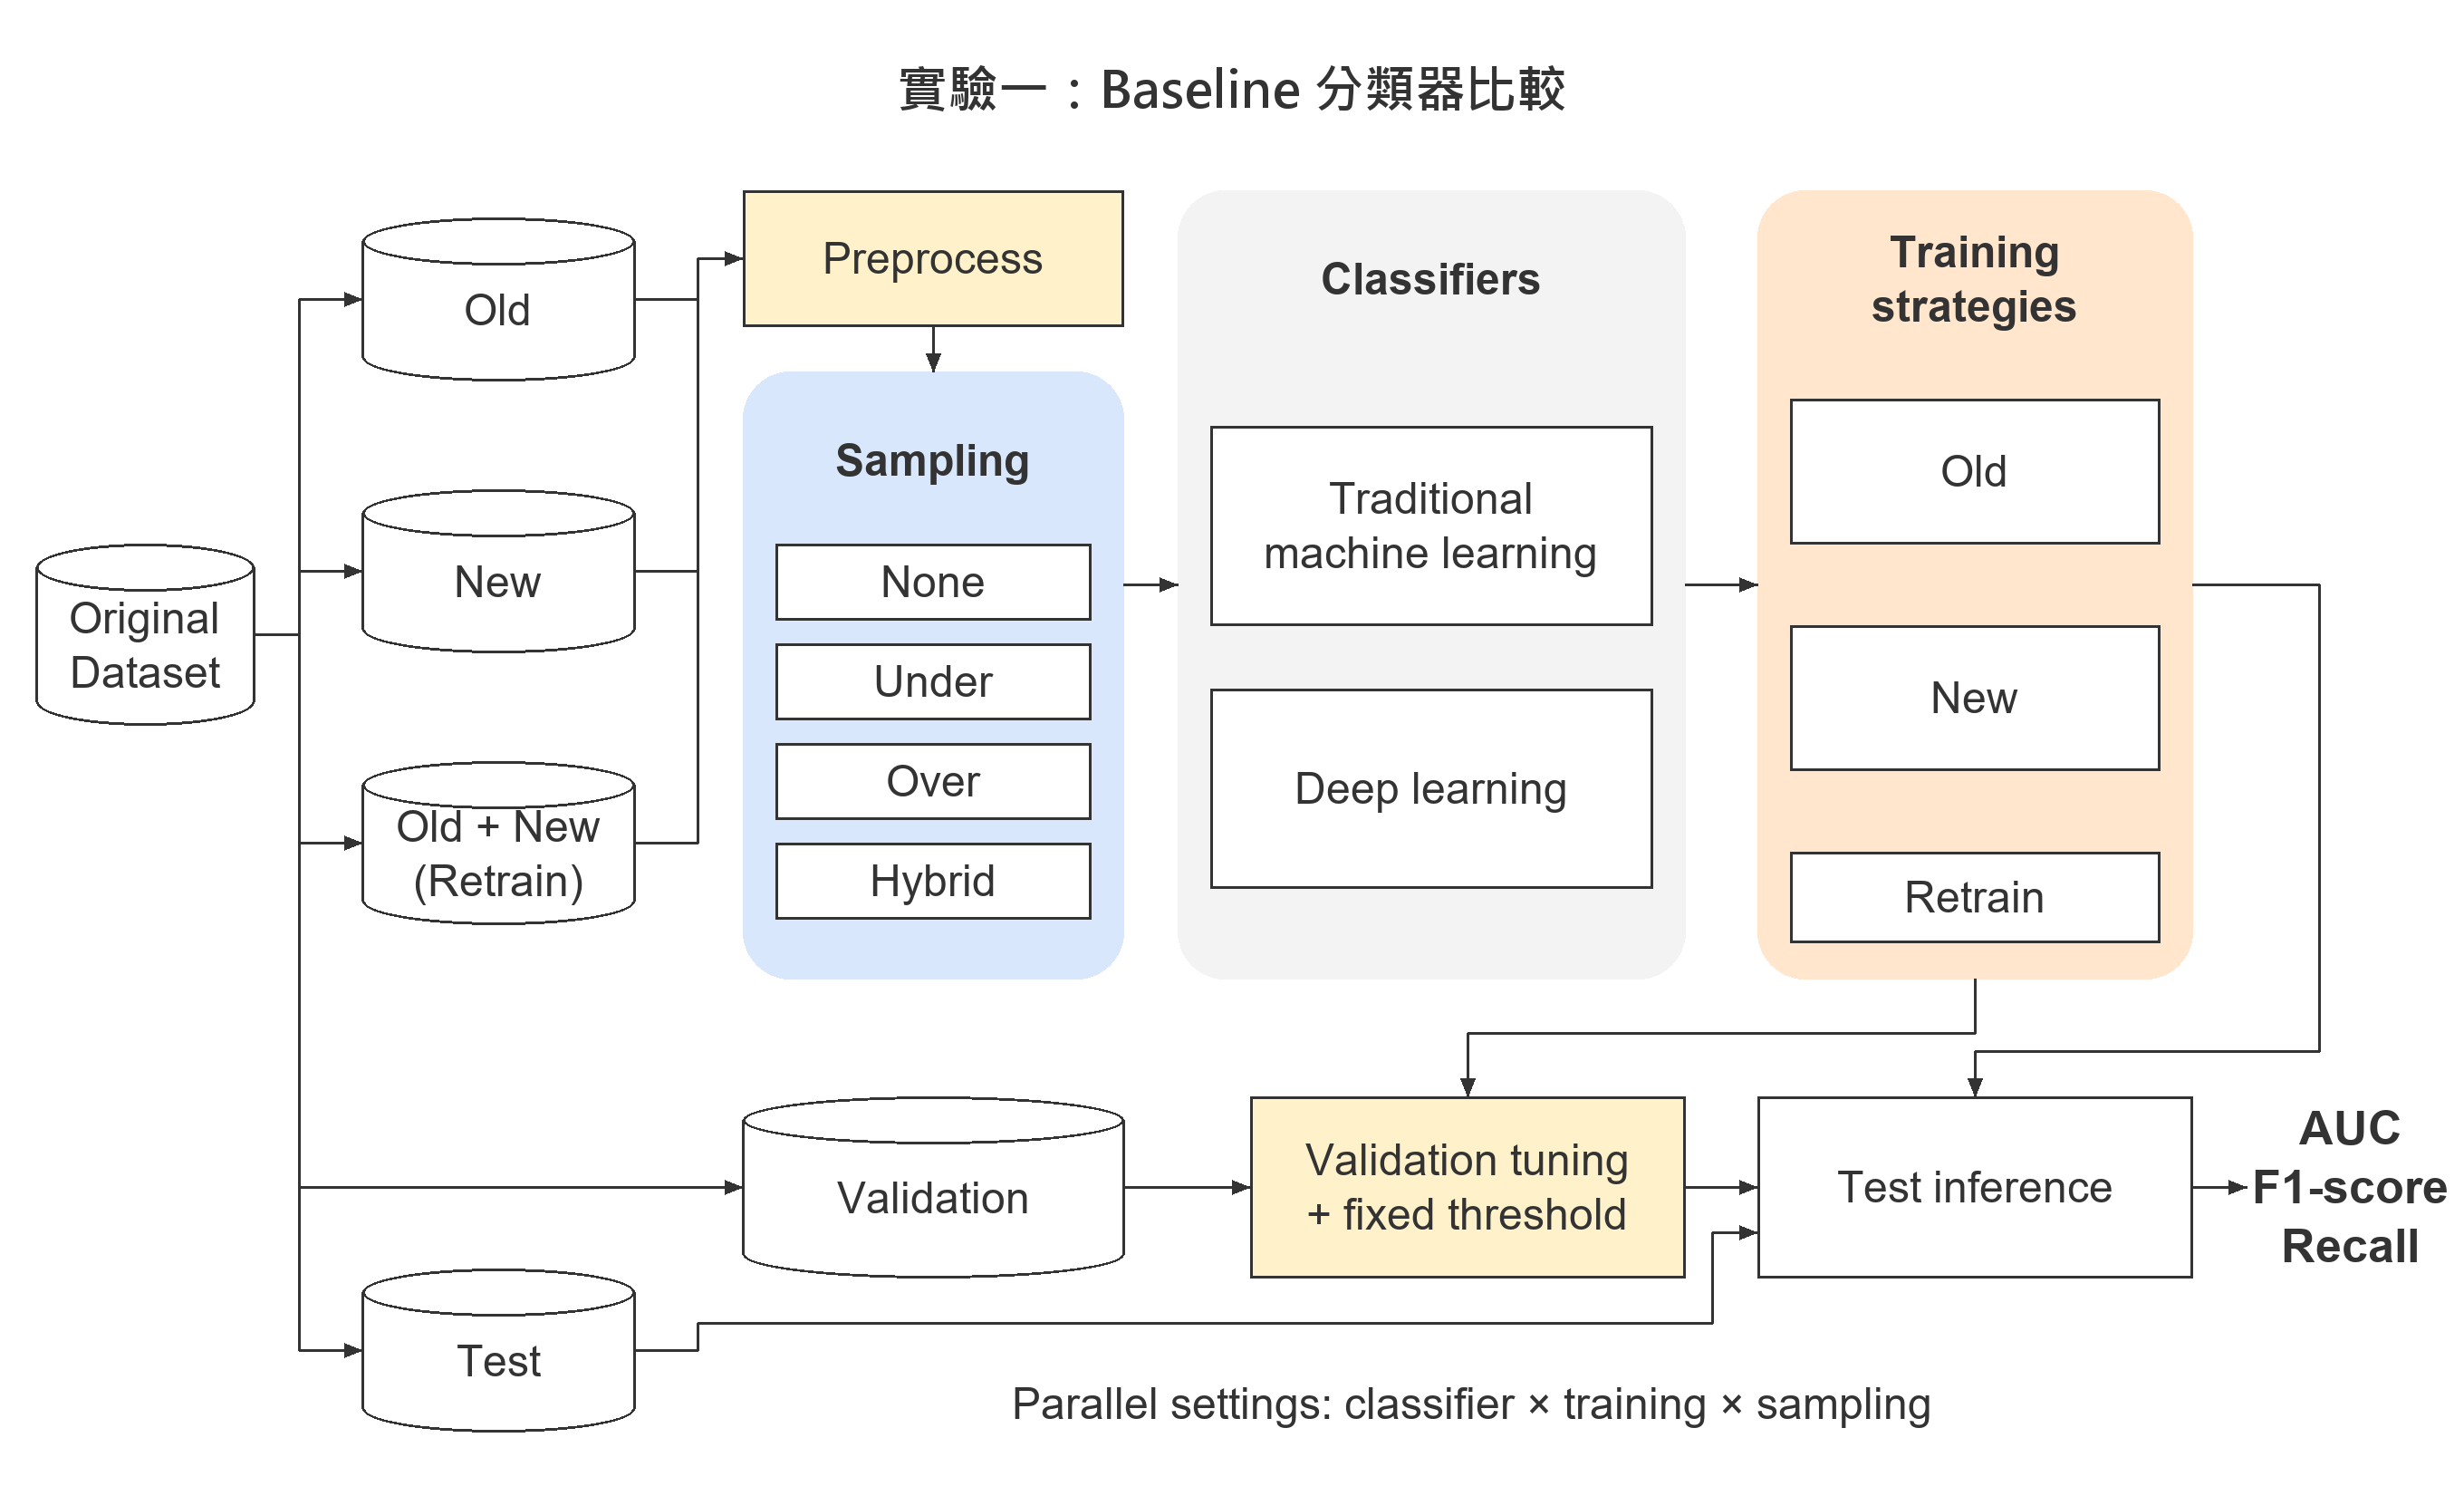
\includegraphics[width=\linewidth]{figures/experiment1-baseline.png}
\caption{實驗一之 Baseline 分類器比較架構}\label{fig:method-baseline}
\par\smallskip{\footnotesize (資料來源：本研究)\par}
\end{figure}





Baseline 與集成使用相同的固定年份：Old 為 1999--2011 年的 Old-fit，New 為 2012--2013 年的 New-fit，Retrain 合併兩者重新訓練單一模型。2014 年全部 3,504 筆紀錄（33 筆事件）作為驗證資料，用於選參與決定門檻；2015--2018 年為 Test。前處理參數只由 Old-fit 估計，與集成實驗相同。

由於驗證事件只有 33 筆，候選間的驗證 AUC 差距可能受少數樣本影響。圖~\ref{fig:method-baseline} 中的深度學習分支涵蓋 TabM 與 TabICL；兩者目前呈現的歷史設定見第~\ref{sec:method-deep-reference}~節，事件數據待更新。

\subsubsection{分類器與訓練策略}

本部分比較三種訓練策略。Old 僅使用歷史期間的擬合資料，評估歷史資訊對較晚年度樣本的適用程度；New 使用近期期間的擬合資料，評估近期資訊所建立的分類能力；Retrain 合併 Old 與 New 的擬合資料，從頭訓練單一模型，作為使用完整可用訓練期間的比較基準。

本章以 New 表示使用近期資料重新訓練的模型，沒有延續舊模型的權重。

\subsubsection{資料前處理與採樣策略}

資料前處理包含平均數補值與標準化，參數只由 Old-fit 估計，再將相同轉換套用於其他分區。

採樣設定包含不採樣（None）、低採樣（Under-sampling）、過採樣（Over-sampling）與混合採樣（Hybrid Sampling）。不採樣保留原始類別分布；其餘設定分別透過樣本刪減、少數類別樣本生成，或兩者結合，改變模型實際使用的訓練資料。採樣僅作用於擬合資料，驗證與測試資料均保留原始類別分布。

本研究採用的代表方法為 TomekLinks、ADASYN 與 SMOTEENN。TomekLinks 依近鄰關係移除類別邊界附近的指定樣本，其作用偏向邊界清理，不能視為固定將兩類樣本調整至相同比例。各方法的參數列於實驗設定，補充版本說明見附錄。

\subsubsection{驗證結果彙整與集成基底定位}

已完成事件標籤部分的比較單位為「分類器 \ensuremath{\times} 訓練策略 \ensuremath{\times} 採樣方式」，共 \(4\times3\times4=48\) 個組合，每個組合以十個種子重做。超參數與門檻固定後，再於 2015--2018 年計算 AUC、F1-score 與 Recall。為了說明集成基底的選擇，第四章另以驗證資料彙整四種分類器在集成池六個位置（Old／New \ensuremath{\times} Under、Over、Hybrid）的表現，不使用 Test 分數。

集成與 FS 實驗以 XGBoost 為固定基底。XGBoost 為樹提升方法\autocite{chen2016xgboost}，其二元機率輸出可直接供靜態平均及動態選擇使用；固定基底也使六模型池只因訓練期間、採樣方式與特徵條件而改變，較容易判讀集成規則與 FS 的影響。此基底在 Baseline 完成前即已決定，並未依 Test 表現回選；本研究也不宣稱 XGBoost 是最佳分類器。

\subsection{Old／New 集成分類器比較}\label{sec:method-phase2}

實驗一的集成部分固定基礎分類器種類，分析不同資料期間與採樣方式所形成模型的整合表現。本部分使用 XGBoost 建立 Old／New 模型池，比較靜態集成、DCS 與 DES，架構如圖~\ref{fig:method-ensemble} 所示。
\begin{figure}[htbp]
\centering
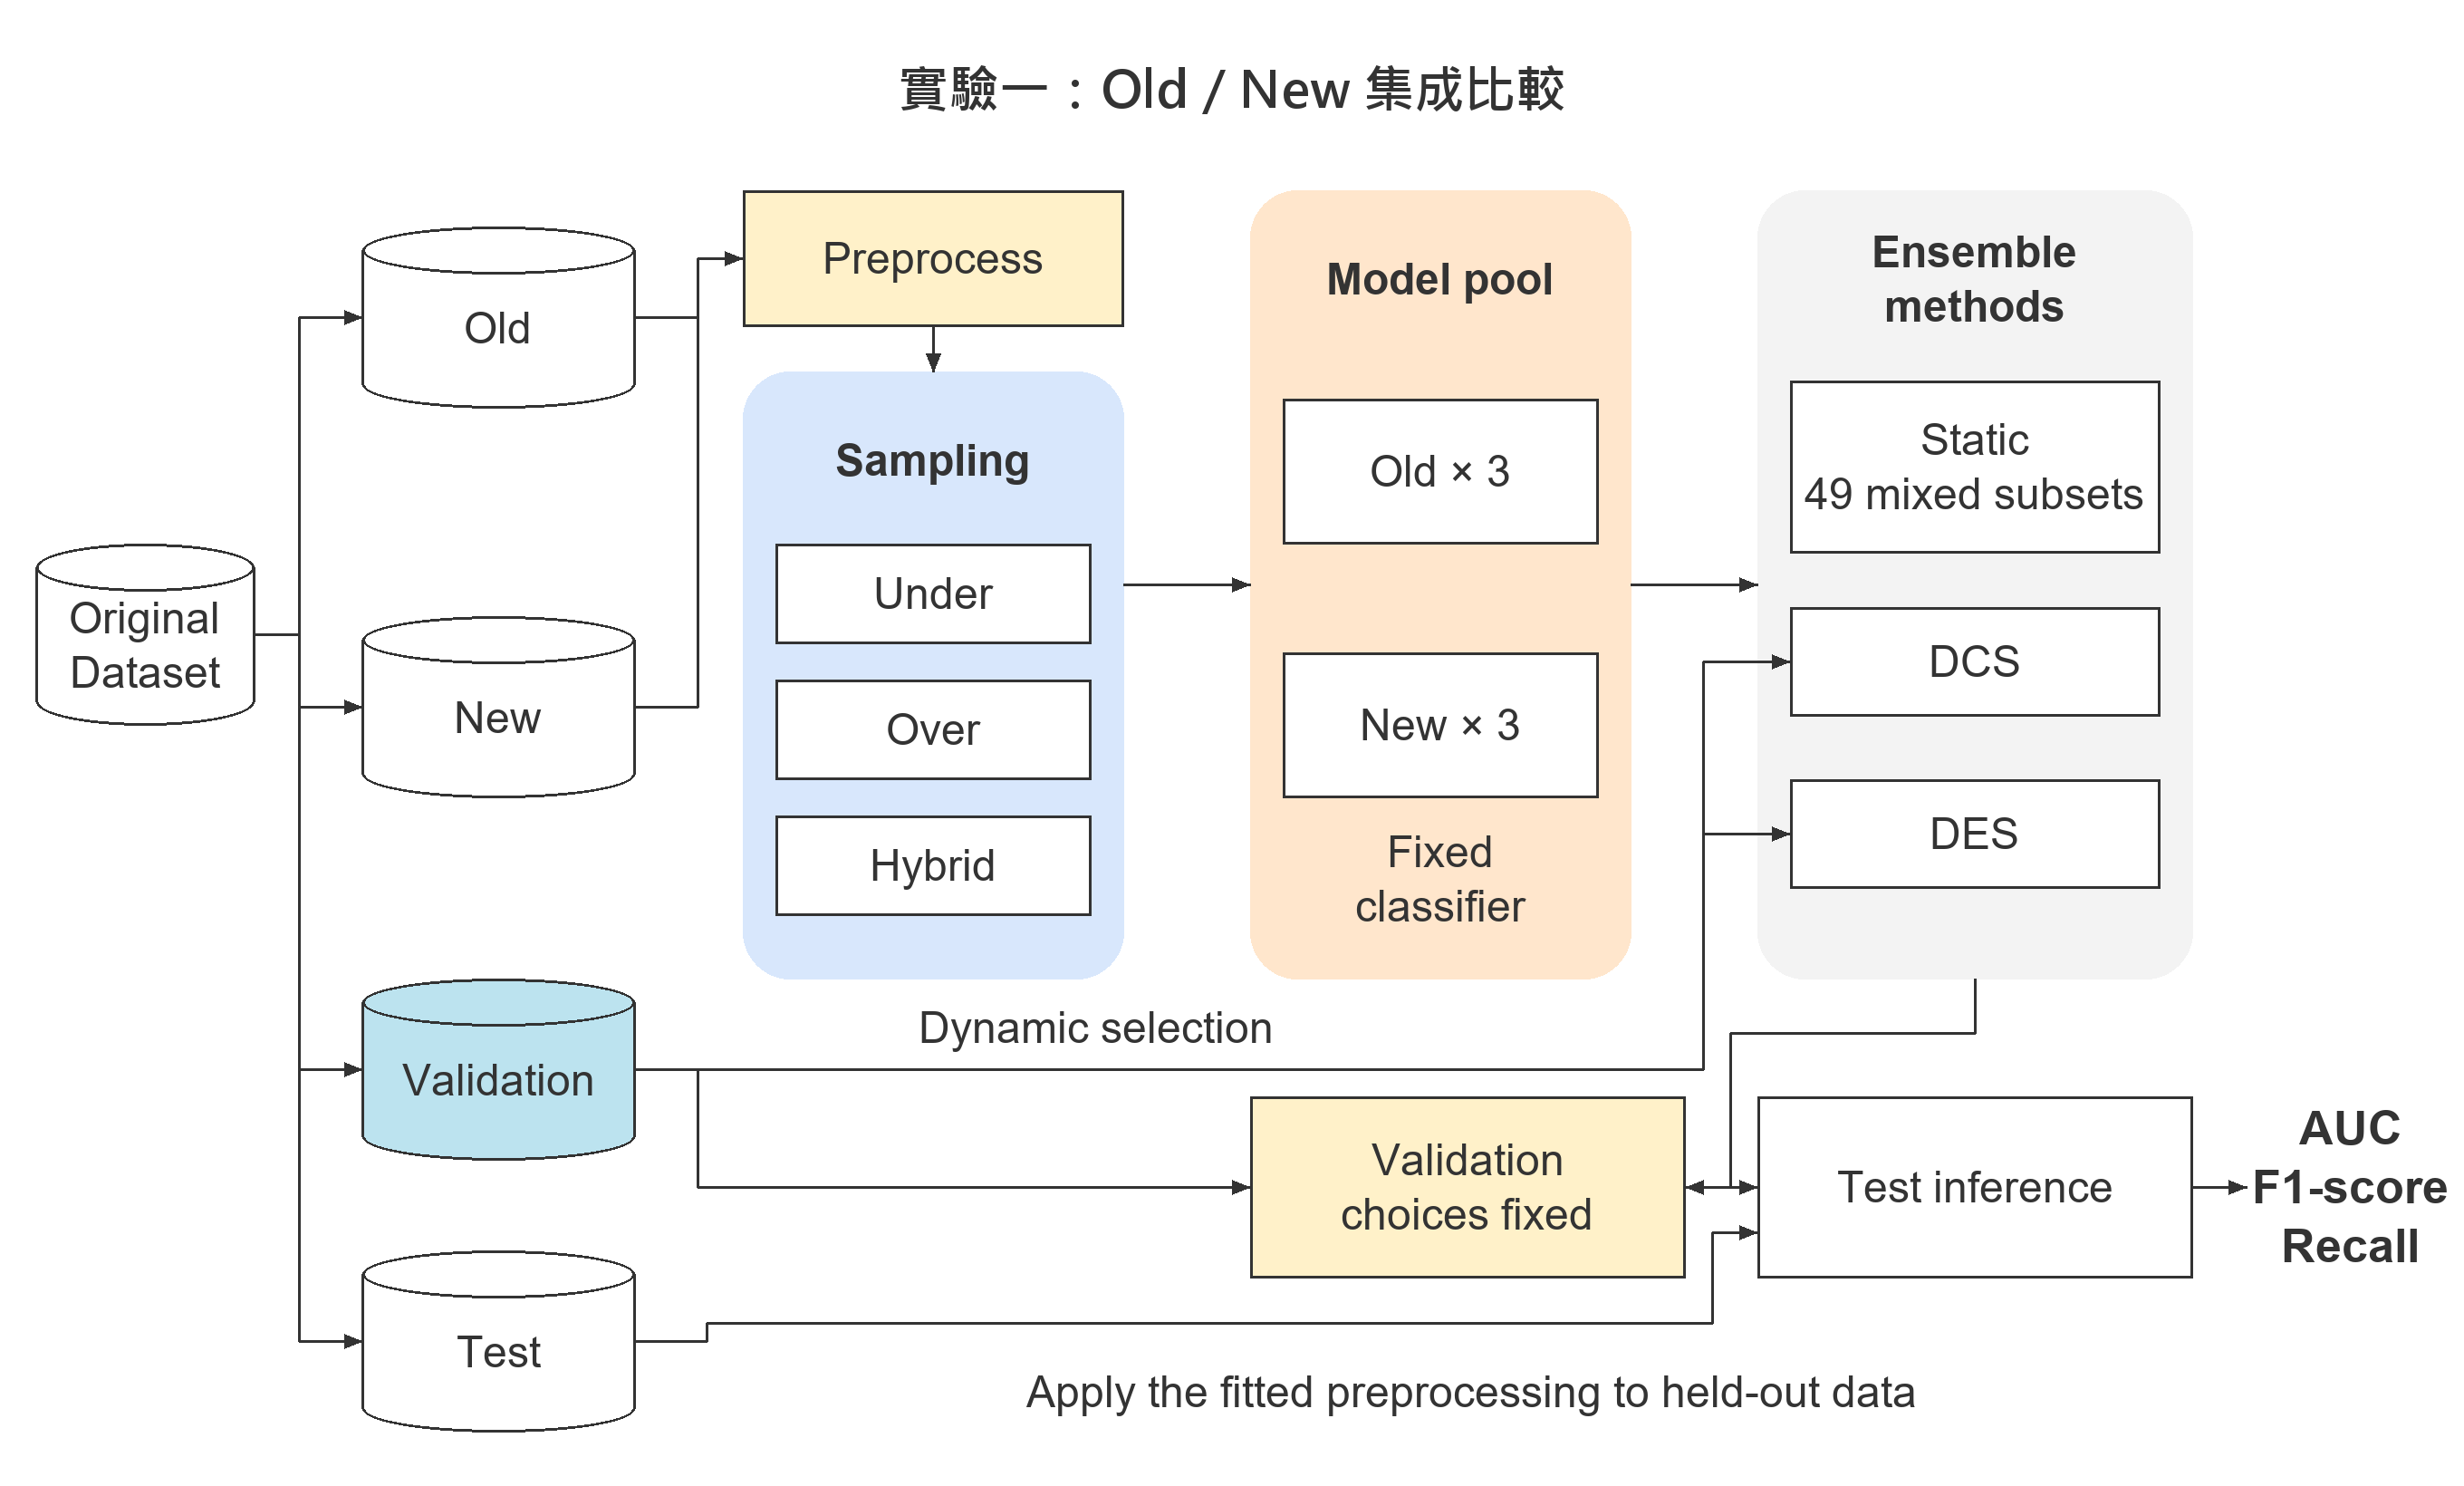
\includegraphics[width=\linewidth]{figures/experiment1-ensemble.png}
\caption{實驗一之 Old／New 集成分類器架構}\label{fig:method-ensemble}
\par\smallskip{\footnotesize (資料來源：本研究)\par}
\par\smallskip{\footnotesize 圖中 Validation 為驗證用途的概括表示；實際分為互不重疊的 DSEL 與 Calibration。前者估計局部分類能力，後者選擇靜態候選及分類門檻。\par}
\end{figure}



\subsubsection{實驗資料切分}

本部分以 1999 年至 2011 年為 Old 訓練期間，2012 年至 2014 年為名義上的 New 營運期間，並固定 2015 年至 2018 年為測試期間。其中，2014 年完整保留供驗證使用，因此 New 模型實際以 2012 年至 2013 年資料進行擬合。

這組界線以原資料研究所使用的 1999--2011、2012--2014 與 2015--2018 年區間為參考\autocite{lombardo2022bankruptcy}，讓各方法都在同一個較晚期間接受測試。本研究將其中 2012--2013 年改供 New 模型學習近期資訊，再保留測試前最近的 2014 年建立 DSEL 與 Calibration。因此，本研究與原文具有相近的年份邊界，但模型可用的訓練資料不同，不直接比較兩者分數。2011 年切點是固定的歷史／近期比較條件，不是由 Test 搜尋得到的最佳年份。

2014 年資料以固定隨機種子 42，依事件標籤分層切分為等量且互不重疊的動態選擇資料集（Dynamic Selection Dataset, DSEL）與校準資料集（Calibration）。DSEL 提供動態方法估計局部分類能力；Calibration 用於靜態候選選擇與分類門檻決定，兩者均不加入基礎分類器的擬合資料。

\input{generated/event-results-20261103/event-partitions.tex}

事件標籤下，DSEL 與 Calibration 各只有 17 與 16 筆事件，靜態成員與門檻的選擇因此較易受少數樣本影響。

Calibration 在本文指用來選擇靜態成員與分類門檻的資料，沒有額外執行機率校準。DSEL 與 Calibration 均取自 2014 年；資料未提供更細的公開時間，兩者只有用途上的區分，沒有年內先後順序。

\subsubsection{基礎模型池建立}

本部分先於 Old-fit 估計各輸入特徵的平均數，以進行遺失值補值，再以補值後的 Old-fit 擬合標準化參數。相同轉換一致套用於 New-fit、DSEL、Calibration 與 Test，使六個基礎模型及動態方法使用共同的特徵表示。

完成前處理後，Old-fit 與 New-fit 各自執行 TomekLinks、ADASYN 及 SMOTEENN，並分別重新訓練分類器，形成表~\ref{tab:method-pool} 所示的六模型池。實驗一之集成比較使用完整 18 個輸入特徵；分類器本身不另加入類別權重，以採樣方式作為本部分的類別不平衡處理因素。

\begingroup
\small
\setstretch{1.15}
\setlength{\tabcolsep}{4pt}
\renewcommand{\arraystretch}{1.25}
\setlength{\LTleft}{0pt plus 1fill}
\setlength{\LTright}{0pt plus 1fill}
\begin{longtable}{@{}>{\raggedright\arraybackslash}p{\dimexpr 0.28\linewidth-1.1200\tabcolsep\relax}>{\raggedright\arraybackslash}p{\dimexpr 0.25\linewidth-1.0000\tabcolsep\relax}>{\raggedright\arraybackslash}p{\dimexpr 0.47\linewidth-1.8800\tabcolsep\relax}@{}}
\caption{Old／New 六模型池組成}\label{tab:method-pool}\\
\toprule
\textbf{模型名稱} & \textbf{擬合資料} & \textbf{採樣方法} \\
\midrule
\endfirsthead
\multicolumn{3}{c}{表~\thetable（續）}\\
\toprule
\textbf{模型名稱} & \textbf{擬合資料} & \textbf{採樣方法} \\
\midrule
\endhead
\midrule
\multicolumn{3}{r}{續下頁}\\
\endfoot
\bottomrule
\endlastfoot
Old\_under & Old-fit & TomekLinks \\
\addlinespace[2pt]
Old\_over & Old-fit & ADASYN \\
\addlinespace[2pt]
Old\_hybrid & Old-fit & SMOTEENN \\
\addlinespace[2pt]
New\_under & New-fit & TomekLinks \\
\addlinespace[2pt]
New\_over & New-fit & ADASYN \\
\addlinespace[2pt]
New\_hybrid & New-fit & SMOTEENN \\*
\end{longtable}
\noindent{\footnotesize (資料來源：本研究整理)}
\endgroup

六個模型都使用 XGBoost，差別在於訓練年度與採樣後的資料。集成比較據此檢查：這些模型的差異是否能補足彼此的預測錯誤。

\subsubsection{集成模型之固定設定}

實驗一的集成部分與實驗二使用相同的 XGBoost 和採樣設定，見表~\ref{tab:method-parameters}；FS 選取器另列於表~\ref{tab:method-fs-parameters}。未另指定的參數沿用固定套件版本預設值。池內 XGBoost 使用預設參數，即 Baseline 搜尋中的候選 0，沒有讀取 Baseline 選定的超參數；兩者的對照列於第~\ref{sec:results-experiment1}~節。

\begingroup
\footnotesize
\setstretch{1.15}
\setlength{\tabcolsep}{4pt}
\renewcommand{\arraystretch}{1.25}
\setlength{\LTleft}{0pt plus 1fill}
\setlength{\LTright}{0pt plus 1fill}
\begin{longtable}{@{}>{\raggedright\arraybackslash}p{\dimexpr 0.2\linewidth-0.4000\tabcolsep\relax}>{\raggedright\arraybackslash}p{\dimexpr 0.8\linewidth-1.6000\tabcolsep\relax}@{}}
\caption{集成模型之主要方法與參數}\label{tab:method-parameters}\\
\toprule
\textbf{項目} & \textbf{固定設定} \\
\midrule
\endfirsthead
\multicolumn{2}{c}{表~\thetable（續）}\\
\toprule
\textbf{項目} & \textbf{固定設定} \\
\midrule
\endhead
\midrule
\multicolumn{2}{r}{續下頁}\\
\endfoot
\bottomrule
\endlastfoot
補值 & Old-fit 平均數補值；保留全空欄位的輸入維度 \\
\addlinespace[2pt]
縮放 & StandardScaler，僅擬合 Old-fit \\
\addlinespace[2pt]
基礎分類器 & XGBoost；{\normalfont objective=\allowbreak{}binary:logistic}、{\normalfont eval\_\allowbreak{}metric=\allowbreak{}auc}、{\normalfont tree\_\allowbreak{}method=\allowbreak{}hist}；預設參數（Baseline 候選 0）；不另加入類別權重，未重新搜尋超參數，亦未啟用早停 \\
\addlinespace[2pt]
低採樣 & TomekLinks；{\normalfont sampling\_\allowbreak{}strategy=\allowbreak{}auto} \\
\addlinespace[2pt]
過採樣 & ADASYN；{\normalfont sampling\_\allowbreak{}strategy=\allowbreak{}auto}、{\normalfont n\_\allowbreak{}neighbors=\allowbreak{}5} \\
\addlinespace[2pt]
混合採樣 & SMOTEENN；SMOTE 的 {\normalfont k\_\allowbreak{}neighbors=\allowbreak{}5}；ENN 的 {\normalfont n\_\allowbreak{}neighbors=\allowbreak{}3}、{\normalfont kind\_\allowbreak{}sel=\allowbreak{}all} \\
\addlinespace[2pt]
靜態候選選擇 & 49 種混合子集，以 Calibration AP 排序；平手依固定方法名稱排序 \\
\addlinespace[2pt]
分類門檻 & Calibration F1-score；0.01–0.99、間隔 0.01；平手取最小門檻 \\
\addlinespace[2pt]
DCS／DES & OLA、LCA、KNORA-E、KNORA-U；{\normalfont k=\allowbreak{}7}、{\normalfont DFP=\allowbreak{}False}、{\normalfont with\_\allowbreak{}IH=\allowbreak{}False}；DCS 使用 {\normalfont best}，DES 使用 {\normalfont soft} \\*
\end{longtable}
\noindent{\footnotesize (資料來源：本研究整理)}
\endgroup

2014 年分區種子固定為 42，所有模型種子與特徵條件均使用相同分區。模型、採樣與具有隨機性的特徵選取程序，使用 42、123、456、789、2024、7、21、84、168、999 共十個種子；可接收種子的元件依各次設定傳遞。Baseline 之超參數候選見表~\ref{tab:method-ml-search}。


軟體環境、補充訓練控制與實驗紀錄規格詳見附錄~\ref{app:experimental-details}。


\subsubsection{靜態集成方法}

靜態集成於推論前固定成員組合，並以成員對正類的預測機率進行等權平均。令模型池中的三個 Old 模型集合為 \(\mathcal{O}\)，三個 New 模型集合為 \(\mathcal{N}\)，則混合候選子集須滿足：

\begin{equation}\label{eq:method-subsets}
S\subseteq\mathcal{O}\cup\mathcal{N},\qquad
S\cap\mathcal{O}\ne\varnothing,\qquad
S\cap\mathcal{N}\ne\varnothing.
\end{equation}

Old 與 New 各有 \(2^3-1\) 個非空子集，因此混合組合數為：

\begin{equation}\label{eq:method-count}
(2^3-1)(2^3-1)=49.
\end{equation}

\begingroup
\small
\setstretch{1.15}
\setlength{\tabcolsep}{4pt}
\renewcommand{\arraystretch}{1.25}
\setlength{\LTleft}{0pt plus 1fill}
\setlength{\LTright}{0pt plus 1fill}
\begin{longtable}{@{}>{\raggedright\arraybackslash}p{\dimexpr 0.55\linewidth-1.1000\tabcolsep\relax}>{\raggedright\arraybackslash}p{\dimexpr 0.45\linewidth-0.9000\tabcolsep\relax}@{}}
\caption{不同模型數量的 Old／New 混合靜態組合}\label{tab:method-combinations}\\
\toprule
\textbf{集成模型數量} & \textbf{混合組合數} \\
\midrule
\endfirsthead
\multicolumn{2}{c}{表~\thetable（續）}\\
\toprule
\textbf{集成模型數量} & \textbf{混合組合數} \\
\midrule
\endhead
\midrule
\multicolumn{2}{r}{續下頁}\\
\endfoot
\bottomrule
\endlastfoot
2 & 9 \\
\addlinespace[2pt]
3 & 18 \\
\addlinespace[2pt]
4 & 15 \\
\addlinespace[2pt]
5 & 6 \\
\addlinespace[2pt]
6 & 1 \\
\addlinespace[2pt]
合計 & 49 \\*
\end{longtable}
\noindent{\footnotesize (資料來源：本研究整理)}
\endgroup

對任一候選子集 \(S\)，集成機率定義為：

\begin{equation}\label{eq:method-probability}
\hat p_S(x)=\frac{1}{|S|}\sum_{i\in S}\hat p_i(x),
\end{equation}

其中，\(\hat p_i(x)\) 為第 \(i\) 個分類器對樣本 \(x\) 預測為正類的機率，\(|S|\) 為該子集的模型數。

除混合候選外，另保留六個單模型，以及三個 Old 模型的等權集成 Old3、三個 New 模型的等權集成 New3，作為比較基準。完整六模型的等權集成稱為 Equal6，其成員組合已包含在 49 種混合候選之中，不額外增加混合組合數。Old3 與 New3 為單一期間控制組，均不納入 49 種跨期間混合候選的選擇範圍。

\subsubsection{動態分類器與集成選擇}

動態選擇依待預測樣本的鄰近區域評估基礎模型的分類能力。本研究以完整六模型池為候選來源，使用獨立 DSEL 建立局部能力估計，並比較動態分類器選擇（Dynamic Classifier Selection, DCS）與動態集成選擇（Dynamic Ensemble Selection, DES）。

DCS 比較 Overall Local Accuracy（OLA）與 Local Class Accuracy（LCA）。OLA 以分類器在樣本鄰近區域的整體正確率估計其能力；LCA 則依各分類器對待預測樣本所判定的類別，估計相應的局部分類能力。兩者原則上選擇局部能力最高的單一分類器，平手時依固定模型順序選擇。

DES 比較 k-Nearest Oracles Eliminate（KNORA-E）與 k-Nearest Oracles Union（KNORA-U）。KNORA-E 尋找能正確分類鄰近區域所有樣本的分類器，必要時縮小鄰域；KNORA-U 則選取至少能正確分類一個鄰近樣本的分類器，並依其局部正確分類次數形成貢獻權重。兩者依所選分類器產生最終集成輸出。

本研究使用 DESlib 0.3.7 的標準實作，鄰居數固定為 \(k=7\)；DES 採機率軟投票，DCS 使用 {\normalfont best} 選擇規則，並關閉額外的動態剪枝與樣本難度分流。當所有基礎分類器對某樣本的類別判斷一致時，沿用套件直接平均機率的處理。因此，DCS 的單分類器選擇描述適用於需要進行局部選擇的情況，不能推定每個樣本的輸出皆來自單一模型。

上述方法的標準定義分別參見 DESlib 的 OLA\autocite{deslib-ola-docs}、LCA\autocite{deslib-lca-docs}、KNORA-E\autocite{deslib-knorae-docs} 與 KNORA-U\autocite{deslib-knorau-docs} 文件；本研究的實際版本與開關設定以正式執行紀錄為準。

\subsubsection{集成候選選擇與分類門檻}

靜態候選與分類門檻均由 Calibration 決定。首先，對 49 種混合靜態候選計算 Calibration AP，選出 AP 最高者，記為 ValidationSelectedStatic。若 AP 相同，依固定的方法名稱字典序決定，以維持選擇結果的可重現性。保留所有候選的測試表現可供組成分析，但不再依 Test 排名回選候選。

其次，各單模型、控制組、靜態候選與動態方法，均在 Calibration 上搜尋 F1-score 最高的分類門檻。門檻候選集合為：

\begin{equation}\label{eq:method-threshold}
\mathcal{T}=\{0.01,0.02,\ldots,0.99\},\qquad
\tau_m^*=\underset{\tau\in\mathcal{T}}{\arg\max}\;
F1_{\mathrm{Calibration}}(m,\tau).
\end{equation}

若多個門檻得到相同的最高 F1-score，採用其中最小者。分類時以 \(\hat p_m(x)\ge\tau_m^*\) 判定為正類；ValidationSelectedStatic 沿用其所選候選的門檻。

候選與門檻固定後，於 Test 計算整體及各年度的 AUC、F1-score 與 Recall。各方法在四個測試年度均沿用相同的 Calibration 門檻，不利用年度測試標籤重新調整。

Retrain 為 Old-fit 與 New-fit 合併訓練的單一模型，不納入六模型池；其結果列於 Baseline，與集成使用相同的資料列與 Test。

\section{實驗二：特徵選取集成分類器比較}\label{sec:method-phase3}

實驗二檢查全部 18 個輸入特徵是否都有保留的必要。資料分區、XGBoost 設定、採樣方式與集成方法沿用實驗一，只在採樣之前加入特徵選取，再重新建立模型池。流程如圖~\ref{fig:method-fs} 所示。
\begin{figure}[htbp]
\centering
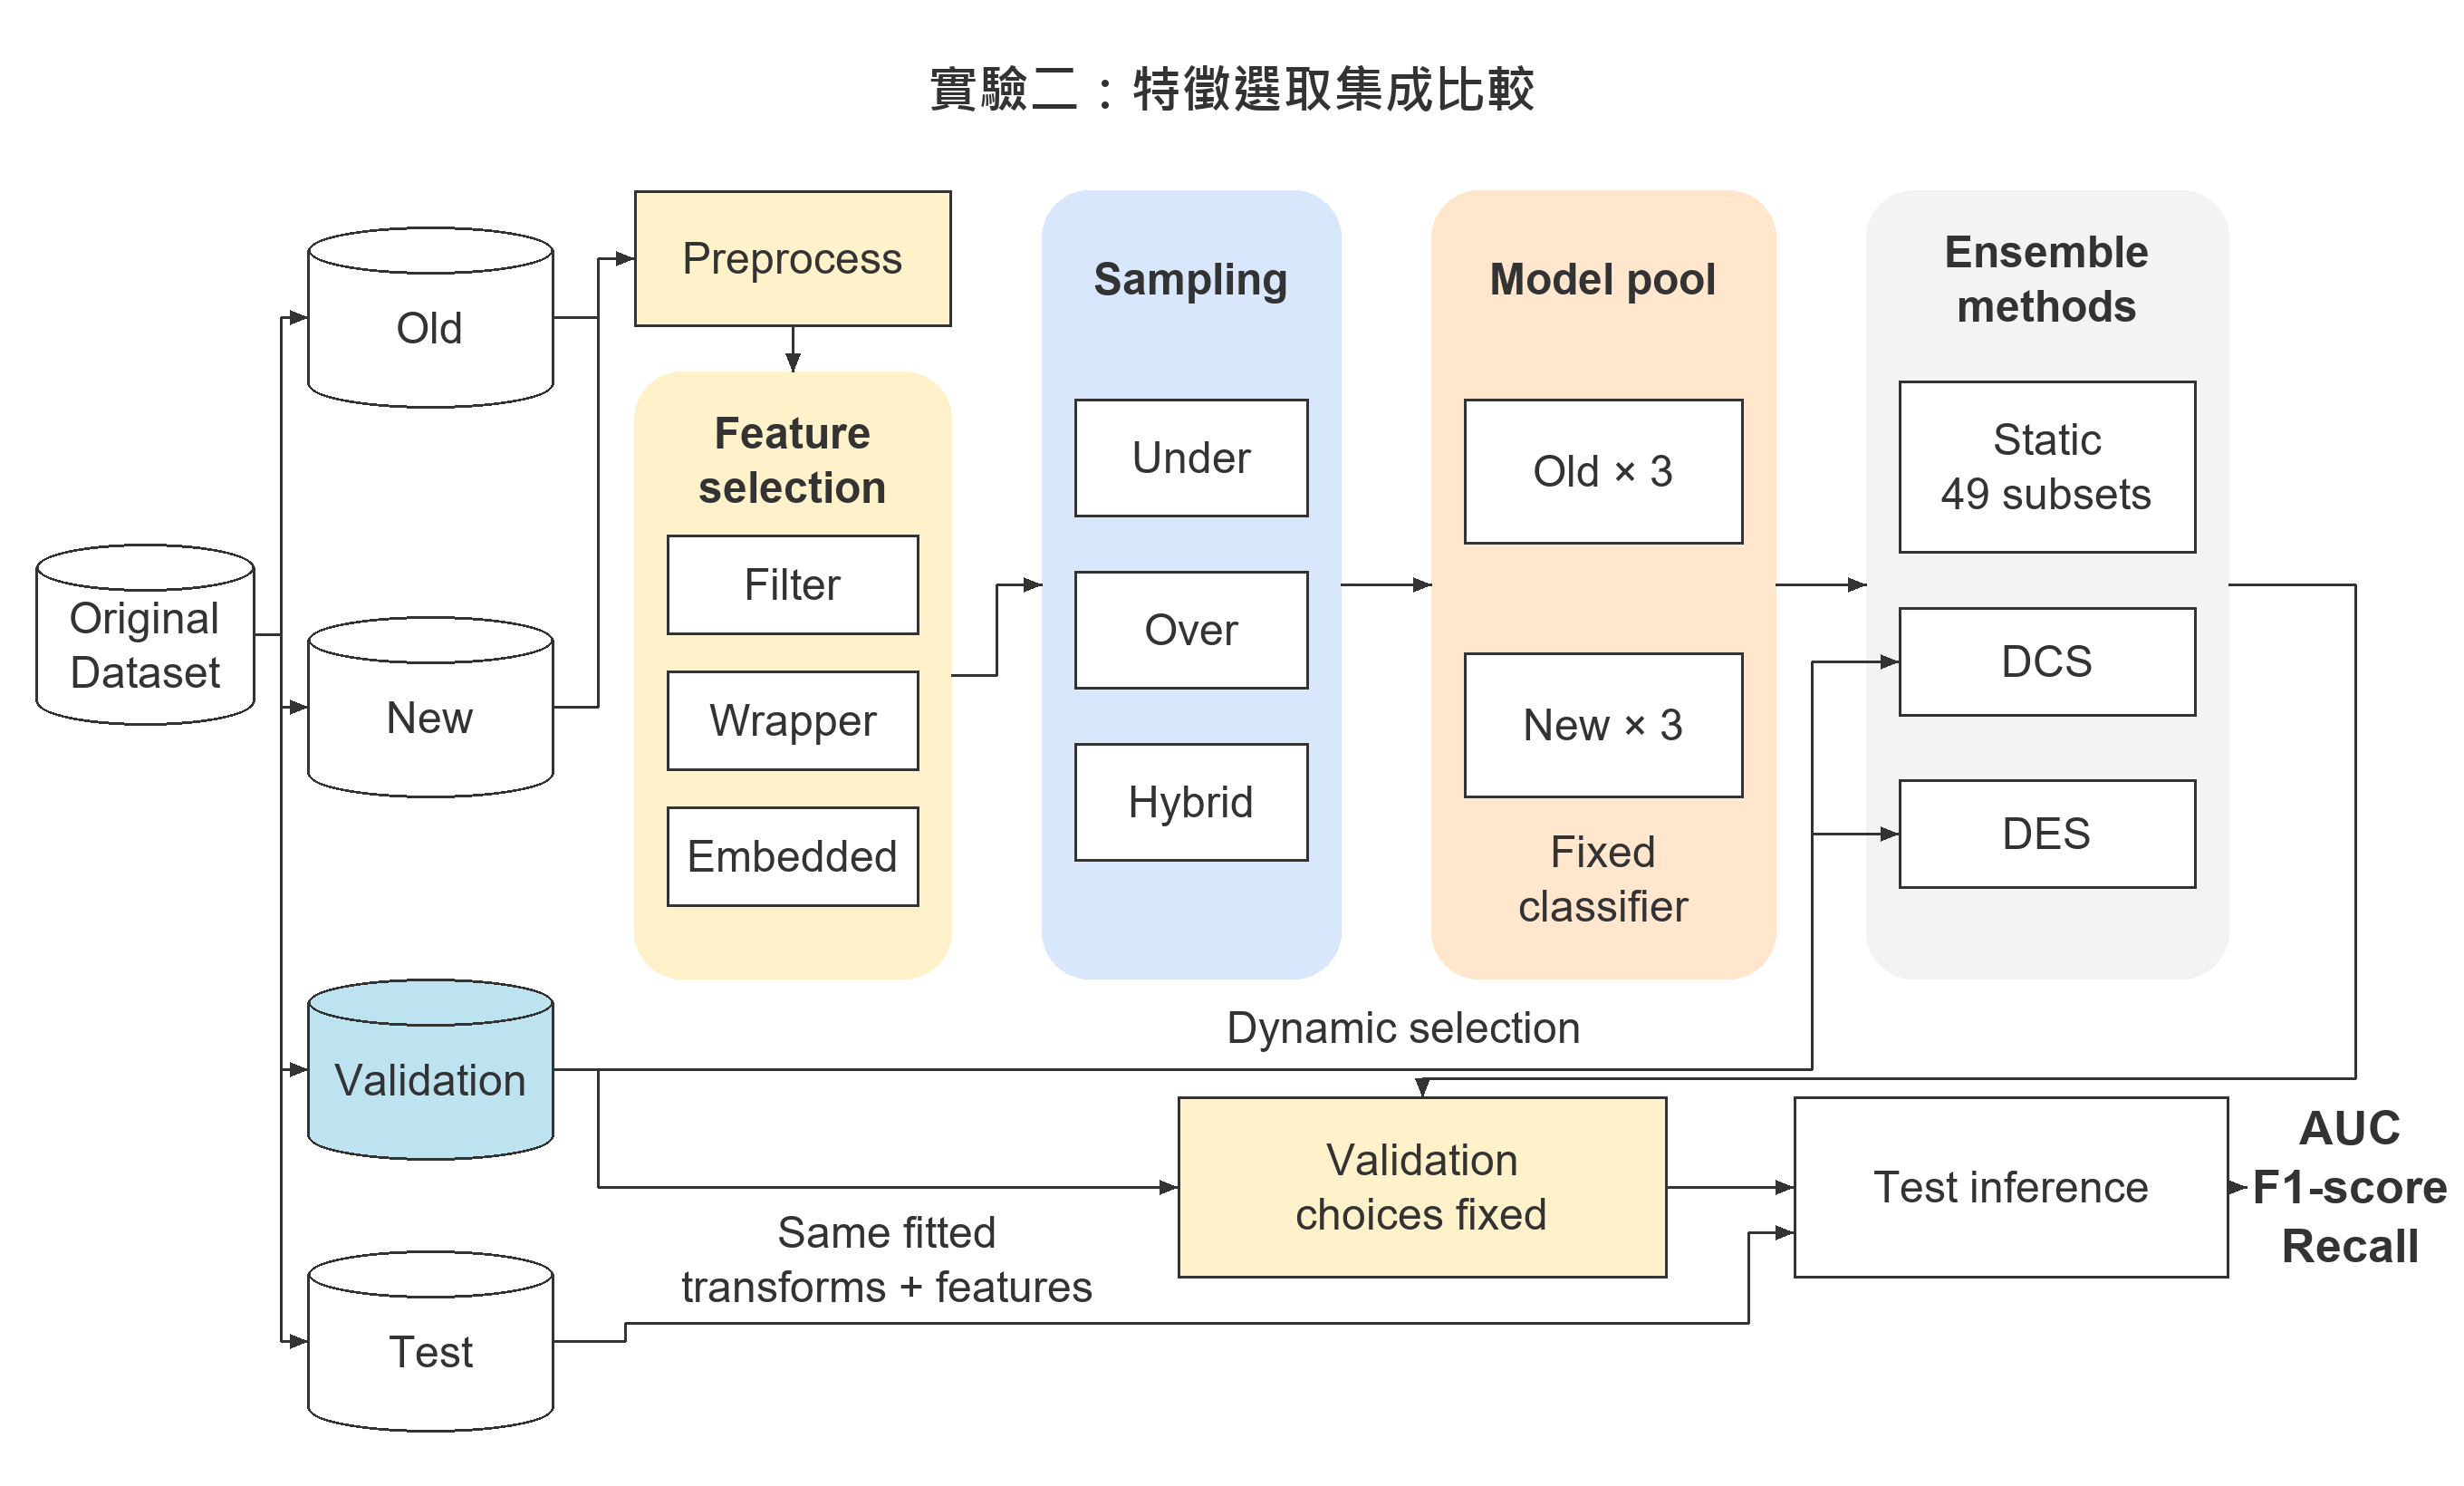
\includegraphics[width=\linewidth]{figures/experiment2-fs-ensemble.png}
\caption{實驗二之特徵選取集成分類器架構}\label{fig:method-fs}
\par\smallskip{\footnotesize (資料來源：本研究)\par}
\par\smallskip{\footnotesize 各 FS 方法平行執行；SHAP 為模型解釋後的特徵排序，其定位另於正文說明。DSEL 與 Calibration 維持實驗一集成部分的分配。\par}
\end{figure}



\subsection{特徵選取方法}

本研究比較 MI、CART、RFE 與 SHAP 排序，操作依據見表~\ref{tab:method-fs}；各方法獨立執行，以 \(k_{\mathrm{FS}}\) 表示保留的特徵數。相關原理與 XAI 的定位已於第二章說明，本節著重實際選取程序。

\begingroup
\small
\setstretch{1.15}
\setlength{\tabcolsep}{4pt}
\renewcommand{\arraystretch}{1.25}
\setlength{\LTleft}{0pt plus 1fill}
\setlength{\LTright}{0pt plus 1fill}
\begin{longtable}{@{}>{\raggedright\arraybackslash}p{\dimexpr 0.15\linewidth-0.6000\tabcolsep\relax}>{\raggedright\arraybackslash}p{\dimexpr 0.28\linewidth-1.1200\tabcolsep\relax}>{\raggedright\arraybackslash}p{\dimexpr 0.57\linewidth-2.2800\tabcolsep\relax}@{}}
\caption{特徵選取方法與操作方式}\label{tab:method-fs}\\
\toprule
\textbf{方法} & \textbf{方法定位} & \textbf{特徵選取依據} \\
\midrule
\endfirsthead
\multicolumn{3}{c}{表~\thetable（續）}\\
\toprule
\textbf{方法} & \textbf{方法定位} & \textbf{特徵選取依據} \\
\midrule
\endhead
\midrule
\multicolumn{3}{r}{續下頁}\\
\endfoot
\bottomrule
\endlastfoot
MI & Filter & 計算各特徵與分類標籤的互資訊，依分數選取前 \(k_{\mathrm{FS}}\) 個特徵 \\
\addlinespace[2pt]
CART & 模型重要性篩選，對應 Embedded 類 & 以決策樹學得的特徵重要性排序，選取前 \(k_{\mathrm{FS}}\) 個特徵 \\
\addlinespace[2pt]
RFE & Wrapper & 以決策樹反覆擬合並移除特徵，直至保留指定數量 \\
\addlinespace[2pt]
SHAP 排序 & 模型解釋後的特徵篩選 & 以 LightGBM 計算訓練樣本的樹模型貢獻值，依平均絕對值排序選取特徵 \\*
\end{longtable}
\noindent{\footnotesize (資料來源：本研究整理)}
\endgroup

MI 與 RFE 由 scikit-learn 實作\autocite{sklearn-fs-docs}。SHAP 排序則使用 LightGBM 的樹模型貢獻值：先排除基準值欄位，再以各特徵的平均絕對貢獻值排序\autocite{lightgbm-booster-docs}。它是模型解釋後的篩選程序，與直接依樹模型重要性選取的 CART 分開比較。

各特徵在十個種子中的入選次數列於附錄，用來描述選取結果的一致性，不另作排名顯著性檢定。

各方法分別設定保留比例 \(r=0.5\) 與 \(r=0.8\)，特徵數依下式決定：

\begin{equation}\label{eq:method-fs-count}
k_{\mathrm{FS}}=\max\{1,\lfloor d\times r\rfloor\},
\end{equation}

其中，\(d=18\) 為原始輸入特徵數。因此，兩種設定分別保留 9 與 14 個特徵；80\% 為名義比例，實際保留數依向下取整規則計算。四種方法各有兩種保留設定，共形成八種特徵選取條件，另以完整 18 特徵作為對照。

50\% 用來觀察刪去約半數特徵的結果，80\% 則代表保留大部分特徵、僅作較小幅度刪減的條件。四種方法共用兩種保留數，可以在相近的特徵數量下比較不同選取規則；no-FS 則提供不刪減特徵的基準。這兩個比例是固定的實驗設計值，沒有依 Calibration 或 Test 最佳化，也不代表所有可能比例中的最適解。

\clearpage
\subsection{實驗二之特徵選取參數}\label{sec:method-fs-parameters}

表~\ref{tab:method-fs-parameters} 列出四種選取器的固定參數及執行規則；未另指定者沿用同版本套件預設值，不使用 Calibration 或 Test 搜尋 FS 參數。

\begingroup
\footnotesize\setstretch{1.12}\setlength{\tabcolsep}{3pt}
\begin{longtable}{@{}>{\raggedright\arraybackslash}p{0.13\linewidth}>{\raggedright\arraybackslash}p{0.31\linewidth}>{\raggedright\arraybackslash}p{0.49\linewidth}@{}}
\caption{實驗二特徵選取之主要參數與執行規則}\label{tab:method-fs-parameters}\\
\toprule
方法 & 參數或項目 & 實際設定 \\
\midrule\endfirsthead
\multicolumn{3}{c}{表~\thetable（續）}\\\toprule
方法 & 參數或項目 & 實際設定 \\
\midrule\endhead
\midrule\multicolumn{3}{r}{續下頁}\\\endfoot
\bottomrule\endlastfoot
\multirow[t]{2}{=}{共同設定} & 擬合資料 & 前處理後的 Old-fit；於採樣前執行 \\*
 & 保留數與隨機種子 & 9、14 個；\nolinkurl{random_state} 隨十個模型種子設定 \\
\multirow[t]{3}{=}{MI} & 函式與連續特徵 & \nolinkurl{mutual_info_classif}；\nolinkurl{discrete_features=auto}，本研究密集數值矩陣按連續特徵處理 \\*
 & 鄰居數 & \nolinkurl{n_neighbors=3}（套件預設） \\*
 & 選取規則 & 互資訊分數由高至低；平手保留原欄位先後順序 \\
\multirow[t]{5}{=}{CART} & 估計器 & \nolinkurl{DecisionTreeClassifier}；\nolinkurl{class_weight=balanced} \\*
 & 分裂規則 & \nolinkurl{criterion=gini}、\nolinkurl{splitter=best}（預設） \\*
 & 樹的大小 & \nolinkurl{max_depth=None}、\nolinkurl{min_samples_split=2}、\nolinkurl{min_samples_leaf=1}（預設） \\*
 & 剪枝與特徵抽樣 & \nolinkurl{ccp_alpha=0}、\nolinkurl{max_features=None}（預設） \\*
 & 選取規則 & 依特徵重要性排序；平手保留原欄位先後順序 \\
\multirow[t]{3}{=}{RFE} & 估計器 & 與 CART 相同的平衡類別權重決策樹 \\*
 & 移除步長及停止條件 & \nolinkurl{step=1}；\nolinkurl{n_features_to_select} 分別為 9、14 \\*
 & 輸出順序 & 依選取遮罩保留原欄位順序 \\
\multirow[t]{6}{=}{SHAP 排序} & 估計器 & \nolinkurl{LGBMClassifier}；\nolinkurl{n_estimators=100}、\nolinkurl{class_weight=balanced} \\*
 & 樹與學習率 & \nolinkurl{boosting_type=gbdt}、\nolinkurl{num_leaves=31}、\nolinkurl{max_depth=-1}、\nolinkurl{learning_rate=0.1}（預設） \\*
 & 葉節點與抽樣 & \nolinkurl{min_child_samples=20}、\nolinkurl{colsample_bytree=1.0}、\nolinkurl{subsample=1.0}（預設） \\*
 & 正則化與執行緒 & \nolinkurl{reg_alpha=0}、\nolinkurl{reg_lambda=0}（預設）；\nolinkurl{n_jobs=4} \\*
 & 重要性計算 & 在 Old-fit 使用 \nolinkurl{pred_contrib=True}；排除基準值欄位，再計算平均絕對貢獻值 \\*
 & 選取規則 & 依貢獻值排序；平手保留原欄位先後順序 \\
\end{longtable}
\noindent{\footnotesize (資料來源：本研究特徵選取程式與固定版本套件設定整理)\par scikit-learn 1.8.0；LightGBM 4.6.0。未列項目沿用相同版本預設值。}
\endgroup

CART、RFE 與 SHAP 排序中的平衡類別權重只用於特徵選取器；後續六個 XGBoost 模型仍依集成實驗的設定訓練。同一種子與 FS 條件選出的特徵會共同套用於六模型及 DSEL。各特徵在十個種子中的入選次數列於附錄~\ref{sec:appendix-data-fs}，供檢視選取結果是否一致。


\subsection{特徵選取與模型訓練流程}

本部分的處理順序固定為「資料分區 \ensuremath{\rightarrow} 前處理 \ensuremath{\rightarrow} 特徵選取 \ensuremath{\rightarrow} 採樣 \ensuremath{\rightarrow} 模型訓練」。補值與標準化參數先以 Old-fit 擬合，再於轉換後的 Old-fit 執行各特徵選取方法。所選特徵及欄位順序固定後，一致套用於 New-fit、DSEL、Calibration 與 Test。

先選特徵再採樣，使選取器看到的是 Old-fit 原始樣本。CART、RFE 的決策樹及 SHAP 排序使用的 LightGBM 仍採平衡類別權重，降低少數類別在特徵評分時被忽略的可能；MI 則直接估計特徵與標籤的互資訊。選取器與後續 XGBoost 基礎模型的參數分開設定，詳見第~\ref{sec:method-fs-parameters}~節。

完成特徵選取後，Old-fit 與 New-fit 分別執行三種採樣，再訓練三個 Old 與三個 New 分類器。各特徵條件均重新建立六模型池，以確保模型於對應的輸入空間中學習。

同一特徵條件下，六模型、DSEL 與其他評估分區都使用相同特徵；換用另一組特徵時，重新建立動態選擇器。刪除部分特徵也可能改變哪些樣本被視為彼此接近，因此 FS 除了影響分類器本身，也可能改變動態方法參考的鄰近樣本。

\subsection{特徵選取後的集成比較}

各特徵條件均沿用實驗一之集成比較的 49 種混合靜態子集、Old3、New3、Equal6 與四種動態方法。DSEL 的資料列分配維持一致；Calibration 分別用於該條件的靜態候選選擇與門檻決定，Test 則使用相同樣本計算最終指標。

FS 與 no-FS 使用相同種子及測試樣本配對。固定方法的比較保持集成規則與模型成員一致；驗證選定靜態集成則在各 FS 條件下重新依 Calibration 選擇成員。後者的差值同時包含特徵選取與靜態成員改變的影響。

對任一固定方法 \(m\) 與指標 \(M\)，配對差值定義為：

\begin{equation}\label{eq:method-delta}
\Delta M_{s,m,f}
=M_{s,m,f}-M_{s,m,\mathrm{no\_fs}},
\end{equation}

其中，\(s\) 表示相同隨機種子，\(f\) 表示特徵選取條件。正值表示該指標高於未進行特徵選取的對照。即使模型成員固定，各條件的分類門檻仍依各自的 Calibration 決定，因此 F1-score 與 Recall 差異反映特徵選取、重新訓練及門檻選擇後的整體結果。除效能外，亦記錄所選特徵名稱、順序與數量，以保留結果追溯依據。

\section{實驗驗證準則}\label{sec:method-validation}

\subsection{訓練、驗證與測試程序}

各部分均先固定資料用途，再執行資料前處理與模型建立。基礎模型的學習、特徵選取及採樣僅使用允許的擬合資料；DSEL 用於動態局部能力估計；Calibration 用於靜態候選及分類門檻決定。測試標籤不參與上述決策。

Calibration 用來比較候選與決定門檻，模型設定已參考過這些資料，因此不能用它的最高分代表最終預測表現。本研究以設定固定後的 Test 結果作正式評估，並保留所有方法與特徵條件，讓讀者可以比較完整結果。

\subsection{分類效能評估指標}

令關注類別為正類。TP 與 TN 分別為正確分類的正類與負類紀錄數；FN 為正類被判為負類的紀錄數；FP 為負類被判為正類的紀錄數。實證案例的正類對應第~\ref{sec:method-data}~節定義的標籤。

\textbf{一、AUC}

ROC 曲線以真陽性率（True Positive Rate, TPR）為縱軸，假陽性率（False Positive Rate, FPR）為橫軸，定義為：

\begin{equation}\label{eq:method-roc}
\mathrm{TPR}=\frac{TP}{TP+FN},\qquad
\mathrm{FPR}=\frac{FP}{FP+TN}.
\end{equation}

AUC 為 ROC 曲線下的面積，用於衡量正負類樣本的排序區辨能力，數值越高表示整體區辨表現越佳。AUC 由預測機率計算，不依賴本研究所選的單一分類門檻；惟其無法單獨反映實際門檻下的正類樣本辨識情形，故另以 F1-score 與 Recall 補充。

\textbf{二、F1-score}

Precision 表示預測為正類的紀錄中，實際正類者所占比例；Recall 表示實際正類紀錄中被正確辨識的比例。兩者與 F1-score 定義如下：

\begin{equation}\label{eq:recall}
\mathrm{Precision}=\frac{TP}{TP+FP},\qquad
\mathrm{Recall}=\frac{TP}{TP+FN},
\end{equation}

\begin{equation}\label{eq:method-f1}
F1=\frac{2\,\mathrm{Precision}\,\mathrm{Recall}}
{\mathrm{Precision}+\mathrm{Recall}}
=\frac{2TP}{2TP+FP+FN}.
\end{equation}

F1-score 同時反映正類預測的精確程度與涵蓋程度。本研究以各方法在 Calibration 決定的門檻計算測試 F1-score；計算遇到未定義的零分母情形時，依統一的評估規則記為零。

\textbf{三、Recall}

Recall 與 TPR 相同，表示實際正類紀錄中被正確辨識的比例。較低的 Recall 代表較多正類紀錄被漏判；惟較高 Recall 亦可能伴隨較多誤報，因此須與 F1-score 及 AUC 共同解讀，不僅依 Recall 判定方法優劣。

\textbf{四、Average Precision}

AP 用於實驗一之集成比較與實驗二的靜態候選選擇，依不同門檻的 Precision 與 Recall 計算：

\begin{equation}\label{eq:method-ap}
\mathrm{AP}=\sum_n(R_n-R_{n-1})P_n,
\end{equation}

其中，\(P_n\) 與 \(R_n\) 分別為第 \(n\) 個操作點的 Precision 與 Recall。本研究以 Recall 增量加權 Precision；此計算不同於對 PR 曲線直接進行梯形積分，定義見 scikit-learn AP 文件\autocite{sklearn-ap-docs}。AP 用於驗證選模，最終主文仍以 AUC、F1-score 與 Recall 為主要報告指標。

\textbf{五、特徵精簡率}

除預測指標外，實驗二也記錄刪除了多少特徵。令原始特徵數為 \(d\)、保留數為 \(k_{\mathrm{FS}}\)，特徵精簡率定義為：
\begin{equation}\label{eq:method-reduction}
R_{\mathrm{FS}}=\left(1-\frac{k_{\mathrm{FS}}}{d}\right)\times100\%.
\end{equation}
原始特徵數為 18，保留 9 個時精簡率為 50.00\%，保留 14 個時為 22.22\%；no-FS 的精簡率為 0\%。名義保留比例為 80\% 的設定，實際保留 14 個，即 77.78\%，因此本文分別報告名義設定與實際數量。本研究未進行獨立的樣本選取實驗，不另套用樣本精簡率解釋過採樣或混合採樣的結果。

\subsection{結果彙整與模型比較}

實驗一的集成比較與實驗二同時呈現整體及逐年結果。整體結果將 2015--2018 年的測試標籤與預測合併，再計算一次指標，以下稱為「合併四年結果（pooled）」。這與先算各年度分數再取平均不同。逐年結果則分開計算每一年的表現，所有年度均沿用驗證時固定的模型與門檻。

相同設定使用十個隨機種子重做，結果以平均值及標準差呈現。標準差越小，表示這十次執行的分數越接近。不過，十次使用的是同一份測試資料，不能當作十份獨立資料來做推論。方法間的統計比較另依第~\ref{sec:method-statistics}~節處理。

實驗一分別比較 Baseline 與固定年份集成；實驗二則在相同種子、方法及測試樣本下，比較有無 FS 的結果。對 V-static 而言，FS 後還會重新選擇模型成員，須與保持成員不變的方法分開解讀。資料切分或訓練規則不同時，分數差可能有多個來源，因此不全部歸因於集成或 FS。本文結論也限於實際使用的資料與年份。

\subsection{以公司為單位的統計比較}\label{sec:method-statistics}

兩個方法的分數不同，可能來自方法本身，也可能與剛好測到哪些公司有關。為了解差異是否穩定，本研究反覆重新抽取測試公司，再比較同一批公司上兩個方法的分數。抽到一家公司時，會一起保留它的各年度紀錄，避免把同一公司的多筆資料當成彼此無關的樣本。

為評估方法間差異的不確定性，本研究分別對事件標籤與最終狀態標籤的固定年份集成結果，補作以公司為重抽單位的配對群聚 bootstrap。兩種標籤各自分析與校正，事件標籤為主要分析，最終狀態標籤為對照。此分析在既有實驗完成後制定，屬事後探索性分析；所有分類器、特徵設定、靜態選模規則與分類門檻均使用已保存的驗證決策，不因檢定結果調整模型。Bootstrap 的一般原理見 Efron 與 Tibshirani\autocite{efron1986bootstrap}；群聚 ROC 資料須考量同一群聚內相關性的原因，見 Obuchowski\autocite{obuchowski1997clustered}。本研究依公司年度資料結構設計下列配對重抽程序。

\subsubsection{比較對象與估計量}

實驗一以完整六模型等權集成 Equal6 為共同基準，分別比較 Old3、New3、驗證選定靜態集成（以下簡稱 V-static）、DCS-OLA、DCS-LCA、KNORA-E 及 KNORA-U，共七組比較。V-static 在各種子內依 Calibration AP 選擇混合成員，不使用 Test 排序結果選擇靜態方案。Baseline 與集成的參數及驗證資料不同，不納入此檢定範圍。

實驗二將 MI、CART、SHAP 與 RFE 的兩種保留比例，各自與相同方法的 no-FS 結果配對。比較方法為 Equal6、V-static、DCS-OLA、DCS-LCA、KNORA-E 與 KNORA-U，因此共有 \(8\times6=48\) 組比較。V-static 允許 FS 後依原有 Calibration 規則重新選擇成員，故該比較評估完整選模程序的變化；其他方法保持方法名稱與規則一致，但仍重新訓練模型並以 Calibration 固定各自門檻。

每組比較均計算 AUC、F1-score 及 Recall，合計 \((7+48)\times3=165\) 項檢定。若 \(M\) 為任一指標，\(S=10\) 為種子數，方法 A 相對方法 B 的差值定義為：
\begin{equation}\label{eq:stats-difference}
\widehat{\Delta}_M=\frac{1}{S}\sum_{s=1}^{S}
\left[M(y,p_{A,s};\tau_{A,s})-M(y,p_{B,s};\tau_{B,s})\right].
\end{equation}
其中，\(p\) 為模型預測機率，\(\tau\) 為驗證程序固定的門檻；AUC 不使用門檻。此估計量先計算各種子的 pooled 指標，再平均其差值，不將十個種子的機率平均後另建一個預測模型。

\subsubsection{重抽、信賴區間與多重比較}

每次 bootstrap 從 Test 所含的 \(C\) 家公司中等機率、有放回抽取 \(C\) 次。公司被抽中後，保留該公司在 2015--2018 年的全部測試紀錄，並將同一組公司抽取次數同時套用於所有種子、方法及 FS 設定。如此可保留同公司跨年的相依性及方法間的配對關係；各次重抽均重新計算指標，但不重新訓練或調整門檻。

事件標籤分析使用 9,999 次重抽，最終狀態標籤對照使用 49,999 次，兩批皆保留既有分析規格，未因顯著性結果改變重抽次數。為使統計分析可重現，bootstrap 重抽樣的隨機種子皆設為 20261027。由差值重抽分布的第 2.5 與第 97.5 百分位數建立逐項 95\% 信賴區間。以 \(\Delta_M^{*(b)}\) 表示第 \(b\) 次重抽差值，針對虛無假設 \(H_0:\Delta_M=0\)，以置中重抽誤差分布計算雙尾近似 \(p\) 值：
\begin{equation}\label{eq:stats-bootstrap-p}
p_M=\frac{1+\sum_{b=1}^{B}\mathbf{1}\!\left\{
\left|\Delta_M^{*(b)}-\widehat{\Delta}_M\right|\geq
\left|\widehat{\Delta}_M\right|\right\}}{B+1},
\qquad B\in\{9{,}999,49{,}999\}.
\end{equation}
式中以有限次隨機重抽估計 \(p\) 值，因此結果仍可能有少量抽樣波動；這種計算也稱為 Monte Carlo 估計。分子與分母各加一，可避免報告零機率；事件標籤與最終狀態標籤的最小可報值分別為 0.0001 與 0.00002。尾端重抽次數很少時，校正後判斷可能對 Monte Carlo 誤差敏感。

同時比較很多方法時，較容易把偶然出現的分數差誤認為有效差異。因此，每一種標籤下的兩項實驗共 165 個 \(p\) 值一併使用 Holm 法\autocite{holm1979multiple} 校正，以降低這類誤判。校正後數值記為 \(p_H\)，小於 0.05 時判為達到統計顯著。表中的 95\% 信賴區間各自計算，沒有作同樣的多重比較校正，所以顯著性仍以 \(p_H\) 為準。未達顯著只表示本次證據不足，不能據此認定兩方法相同。

上述分析固定原有模型、資料切分與驗證決策，只改變抽到的測試公司。因此，它回答的是「換一批測試公司時，兩方法的分數差是否仍相近」，沒有評估換一批訓練資料後的變化。此外，不同公司也可能受到相同產業或景氣影響，這些關聯未另行估計。結果應限於本次資料與設定解讀。事件標籤的檢定於第~\ref{sec:results-event-statistics}~節摘要，兩種標籤的完整比較分列於附錄。
\endgroup
